\section{Theoretical Analysis}
\label{sec:analysis}

In this section, the circuit shown in Figure~\ref{fig:rc} is analysed
theoretically, using both mesh and node analysis.
Here, we lay out the background information that was essential for the execution of this assignment. Since the circuit at hand is a simple one we only needed the following information (this is all referenced in Horowitz, P; Hill,W(2015). The Art of Electronics. Cambridge University Press(3rd ed, pp.2-4)):
The sum of the currents into a point in a circuit equals the sum of the currents out. Each of these points is referred to as a node. This is also known as Kirchhoff’s current law (KCL).
The sum of the voltage drops around any closed circuit is zero.This is Kirchhoff’s voltage law (KVL).
The power consumed by a circuit device is
\begin{equation}
  P=VI;
\end{equation}

When voltages and currents are in the same direction they produce a positive power (the component is consuming energy). Voltages and currents in opposite direction produce negative power (the component is giving forth energy to the circuit)
A resistor is characterized by its resistance:
\begin{equation}
  R=\frac {V}{I};
\end{equation}
This is known as Ohm’s law.
Independent V/I sources impose voltage/current regardless of current/voltage.
Linearly dependent V/I sources impose voltage/current that is linearly dependent on a specific variable of other circuit component.

The circuit consists of four independent meshes, and 11 branches where different currents circulate. These will be our variables in the mesh analysis. The current flow is depicted in Figure ~\ref{fig:current}


The components we are working with have a linear relationship between the voltage and current, therefore we will need to solve a system of linear equations to determine the variables of each component given some initial values.
We will use two different methods that are based on KCL and KVL. These methods are the Mesh and Node methods. Each one of them will produce its set of equations that when solved, will give  us either the currents flowing through each mesh (Mesh Method) or the voltage on each node (Node Method).
We’ve written a program on GNU Octave to help us determine the solution for the linear system. The simulation of the circuit was carried out by the Ngspice tool. We’ve written a simple code describing the circuit.

\begin{figure}[h] \centering
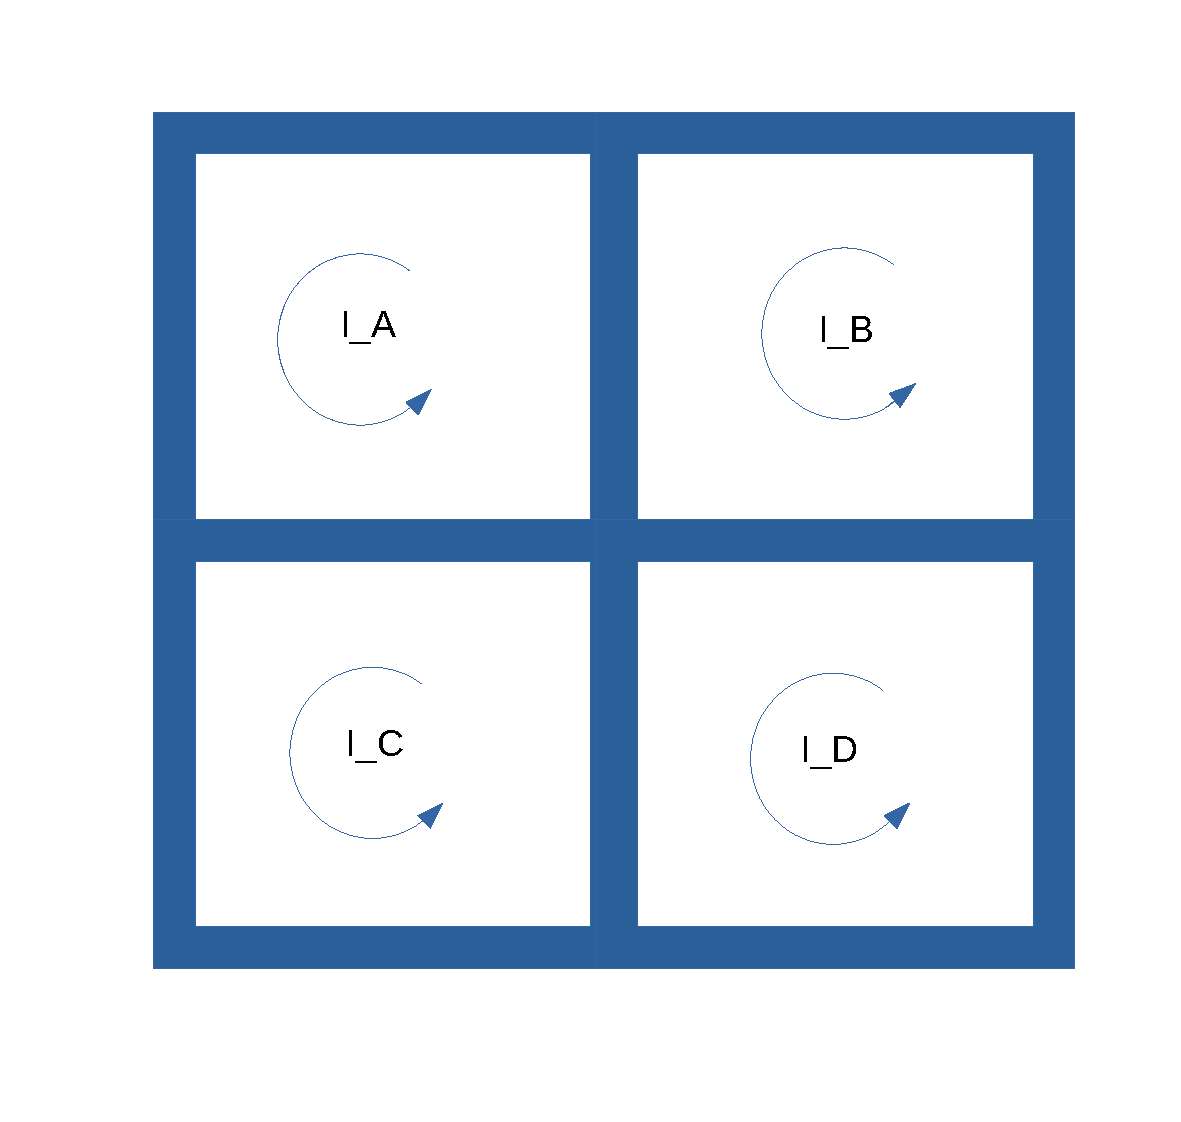
\includegraphics[width=0.4\linewidth]{current.pdf}
\caption{Direction of each mesh current.}
\label{fig:current}
\end{figure}

\subsection{Mesh Analysis}

\begin{figure}[h] \centering
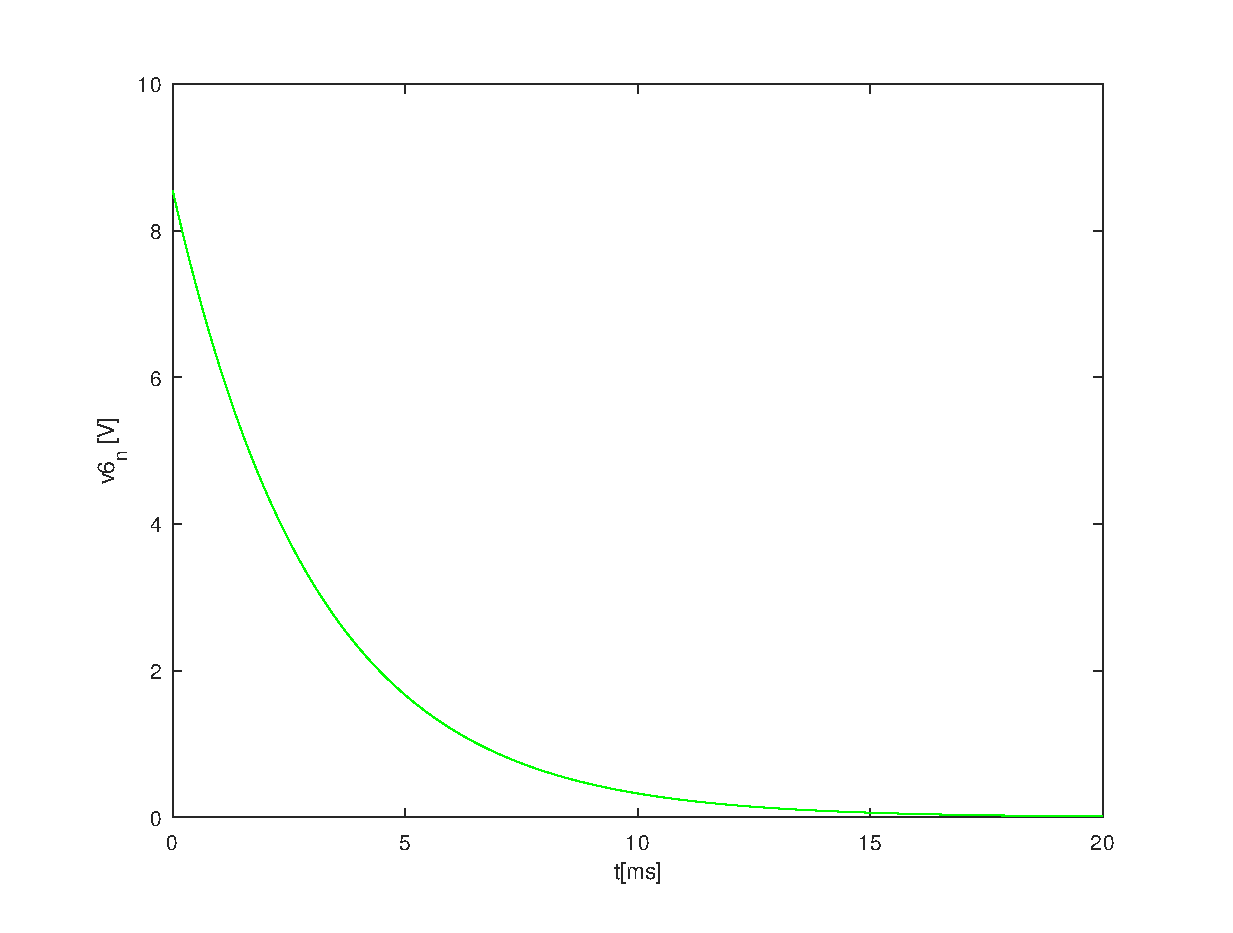
\includegraphics[width=0.8\linewidth]{natural.eps}
\caption{Natural solution to $V_{6}$ node voltage.}
\label{fig:current}
\end{figure}

\begin{figure}[h] \centering
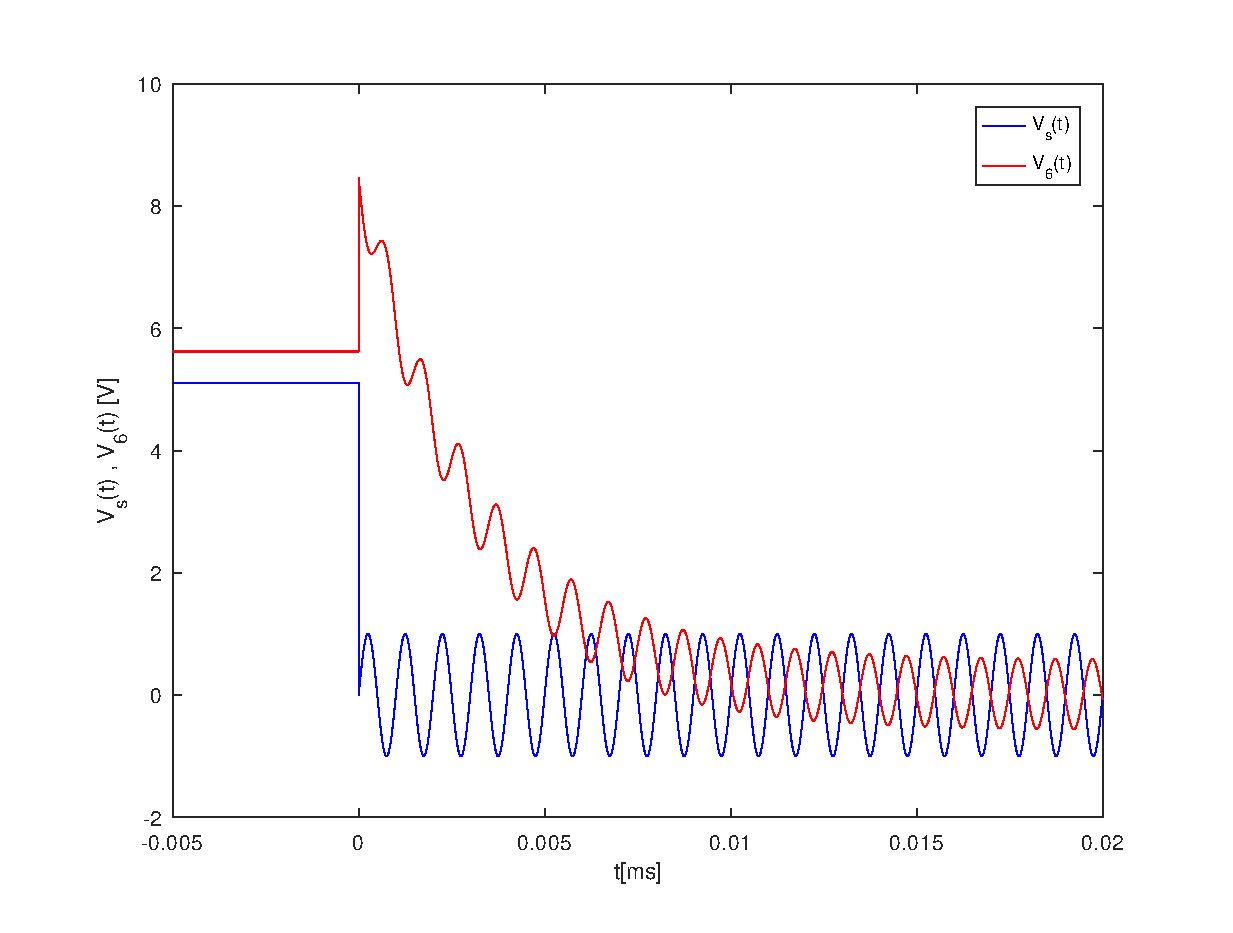
\includegraphics[width=0.8\linewidth]{total.eps}
\caption{Total solution to $V_{6}$ node voltage.}
\label{fig:current}
\end{figure}

Applying the Kirchhoff Voltage Law (KVL) in the different loops, we get four different equations, which we can then solve as a matrix:
\begin{equation}
  I_D=I;
\end{equation}

\begin{equation}
  (R_1+R_3+R_4)I_A-R_3I_B-R_4I_C=-V_A;
\end{equation}

\begin{equation}
  (R_4+R_6+R_7-K_C)I_C-R_4I_A=0;
\end{equation}

\begin{equation}
  (R_3K_B-1)I_B-R_3K_BI_A=0.
\end{equation}

\begin{equation}
\begin{pmatrix}
0 & 0 & 0 & 1 \\
R1+R3+R4 & -R3 & -R4 & 0 \\
-R4 & 0 & R4+R6+R7-Kc & 0 \\
-R3Kb & R3Kb-1 & 0 & 0
\end{pmatrix}
\begin{pmatrix}
Ia\\
Ib\\
Ic\\
Id
\end{pmatrix}
=
\begin{pmatrix}
I\\
-V\\
0\\
0
\end{pmatrix}
\end{equation}



\begin{table}[h]
  \centering
  \begin{tabular}{|l|r|}
    \hline    
    {\bf Name} & {\bf Value [A]} \\ \hline
    @$I_{a}$ & 0.000834 \\ \hline 
@$I_{b}$ & 0.000875 \\ \hline 
@$I_{c}$ & -0.000330 \\ \hline 
@$I_{d}$ & 0.000000 \\ \hline 
 
  \end{tabular}
  \caption{Theoretical analysis results from Octave. (A variable preceded by @ is of type {\em current})}
  \label{tab:mesh}
\end{table}

\subsection{Node Analysis}

As in the previous section, we extract a set of equations from the circuit, this time using the node method. This yields 8 equations, one for each node. Then, we can solve those 8 equations in the form of the matrix presented here.
\begin{equation}
\begin{pmatrix}
G7 & 0 & 0 & 0 & 0 & 0 & G6 & 0\\
1 & -1 & 0 & 0 & 0 & 0 & 0 & 0\\
0 & 0 & 0 & 0 & 0 & 1 & -1 & 0\\
0 & 0 & 0 & -G2 & G1+G2+G3 & -G1 & 0 & -G3\\
0 & 0 & G5 & 0 & G3 & 0 & G4+G6 & -G3-G4-G5\\
1 & 0 & 0 & 0 & 0 & 0& Kc*G6 & -1\\
0 & 0 & 0 & 0 & G1 & -G1 & -G4-G6 & G4\\
0 & 0 & 0 & -G2 & Kb+G2 & 0 & 0 & -Kb
\end{pmatrix}
\begin{pmatrix}
V1\\
V2\\
V3\\
V4\\
V5\\
V6\\
V7\\
V8
\end{pmatrix}
=
\begin{pmatrix}
0\\
0\\
V\\
0\\
I\\
0\\
0\\
0
\end{pmatrix}
\end{equation}

\begin{table}[h]
  \centering
  \begin{tabular}{|l|r|}
    \hline    
    {\bf Name} & {\bf Value [V]} \\ \hline
    $V_{1}$ & 5.113399 \\ \hline 
$V_{2}$ & 4.260917 \\ \hline 
$V_{3}$ & 2.507106 \\ \hline 
$V_{4}$ & -0.000000 \\ \hline 
$V_{5}$ & 4.382714 \\ \hline 
$V_{6}$ & 7.045254 \\ \hline 
$V_{7}$ & -0.667990 \\ \hline 
$V_{8}$ & -1.000947 \\ \hline 
 
  \end{tabular}
  \caption{Theoretical analysis results from Octave.}
  \label{tab:node}
\end{table}
